%File: focus_paper.tex
\documentclass[letterpaper]{article}


% Required Packages
\usepackage{aaai}
\usepackage{times}
\usepackage{helvet}
\usepackage{courier}
\usepackage{graphicx}
\usepackage{url}
\usepackage{listings}
\usepackage{graphicx}
\usepackage{verbatim} % used to display code
\usepackage{hyperref}
%\usepackage{fullpage}
\usepackage[ansinew]{inputenc} % german umlauts
\usepackage[usenames,dvipsnames]{color}
\usepackage{float}
\usepackage{subfig}
\usepackage{tikz}
\usetikzlibrary{calc,through,backgrounds}
\usepackage{fancyvrb}
\usepackage{acronym}
\usepackage{amsthm} % Uuhhh yet another package
\VerbatimFootnotes % Required, otherwise verbatim does not work in footnotes!
%\usepackage{listings}

\definecolor{Brown}{cmyk}{0,0.81,1,0.60}
\definecolor{OliveGreen}{cmyk}{0.64,0,0.95,0.40}
\definecolor{CadetBlue}{cmyk}{0.62,0.57,0.23,0}
\definecolor{lightlightgray}{gray}{0.9}

\begin{document}

\lstset{
language=bash,                          % Code langugage
basicstyle=\ttfamily,                   % Code font, Examples: \footnotesize, \ttfamily
keywordstyle=\color{OliveGreen},        % Keywords font ('*' = uppercase)
commentstyle=\color{gray},              % Comments font
numbers=left,                           % Line nums position
numberstyle=\tiny,                      % Line-numbers fonts
stepnumber=1,                           % Step between two line-numbers
numbersep=5pt,                          % How far are line-numbers from code
backgroundcolor=\color{lightlightgray}, % Choose background color
frame=none,                             % A frame around the code
tabsize=2,                              % Default tab size
captionpos=b,                           % Caption-position = bottom
breaklines=true,                        % Automatic line breaking?
breakatwhitespace=false,                % Automatic breaks only at whitespace?
showspaces=false,                       % Dont make spaces visible
showtabs=false,                         % Dont make tabls visible
columns=flexible,                       % Column format
morekeywords={__global__, __device__},  % CUDA specific keywords
}

%%%%%%%%%%
% Pdfinfo for PDFTEX
% Uncomment and complete the following for metadata if % your paper is
% typeset using PDFTEX
\pdfinfo{
/Title (The Feasibility of Stylometry as a Service)
/Author (Josh Datko and Joseph Heenan)
/Subject (The Feasibility of Stylometry as a Service)
/Keywords (privacy anonymity stylometry )
}
%%%%%%%%%%
% Section Numbers
% Uncomment if you want to use section numbers
% and change the 0 to a 1 or 2
\setcounter{secnumdepth}{1}
%%%%%%%%%%
% Title, Author, and Address Information
\title{The Feasibility of Stylometry as a Service}
\author{Josh Datko \and Joseph Heenan\\ Drexel University\\
CS680: Privacy in the Electronic Society\\
}
%%%%%%%%%%
% Body of Paper Begins \begin{document}
\maketitle

\section*{Introduction}\label{sec:intro}


Maintaining anonymity online is increasingly difficult.  While
networks like Tor \cite{Dingledine04tor:the} will protect an Internet
Protocol (IP) address at the network layer, it does not protect the
content delivered over Tor.  For example, suppose an author desires to
provide controversial political commentary but wants to remain
anonymous.  In this case, she can protect her IP address with Tor and
use end-to-end encryption to protect her message en-route, but she
could be discovered through stylometry.

Stylometry, a form of authorship recognition, has been found to be
extremely effective especially even at
Internet-scale \cite{Narayanan:2012:FIA:2310656.2310687}.  Thus for
those seeking to publish anonymous writings, not only can the delivery
path reveal them, but their content can as well.  Adversarial
stylometry is the active process of manipulating writing to confuse
the identity of the author.  A set of tools, JStylo and
Anonymouth \cite{conf/pet/McDonaldACSG12}, have been produced by the
Privacy, Security, and Automation Lab (PSAL) at Drexel University to
assist authors in anonymize their writing.

Currently the JStylo and Anonymouth integrated open-source project
(JSAN) \cite{BrennanG09}, \cite{journals/tissec/BrennanAG12},
\cite{conf/pet/McDonaldACSG12} is available to download and can be
installed on a machine that runs the Java Virtual Machine (JVM).
While JSAN has been successfully demonstrated to be effective in
assisting authors with adversarial stylometry
\cite{journals/tissec/BrennanAG12}, the constraint of downloading and
installing the software on a machine powerful enough to run machine
learning algorithms on data sets, limits their adoptability.  We
propose increase the availability and usability of JStylo and
Anonymouth by offering them as a web service.

Migrating to a web service would provide JSAN with several benefits.
This web service would provide adversarial stylometry capabilities to
embedded devices like tablets or smart-phones which otherwise could
not run the software natively.  Since there would be no installation,
besides a typical web-browser, a web-service would be better suited
for time-critical situations where an author must quickly anonymize
her document.

An example use-case is an author with a time sensitive document that
she needs to release.  Because of the sensitive nature, she wishes to
apply adversarial stylometry to her document.  In this case, a
computer with decent enough performance to natively run machine
learning techniques may not be available.  However, a web service is
nearly ubiquitous.

\subsection{Expanding Stylometric Research}

A stylometric web service also expands research opportunities.  This
service, offered through a modern architecture, would allow
researchers to easily perform experiments.  An easily accessible tool
allows for rapid verification of research results and greater
community engagement.

In addition to convenient access, a web service can provide additional
diversity in stylometric experimentation.  For example, this web
service supports multiple authors and provides a better tool for
real-time, multiple author stylometry than a stand-alone application.

An effective technique in adversarial stylometry is imitation of
another author's writing style.  However, since many are not trained
author imitators, this technique requires significant cognitive effort.
Perhaps a more effective technique, would be to have multiple authors
re-write the target work in their natural style.  While there has been
numerous studies into single author stylometric analysis, multiple
authorship is more difficult.  This web services provides a platform
for multiple authorship research.

\subsection{Challenges in a Web Service}

A privacy enhancing technology that is designed to exist as a web
service faces different challenges than an application.  Attack
vectors open up on the service from active denial-of-service attacks
to passive sniffing.  A privacy web service must take great care to
ensure that service does not compromise its user's privacy.  In
Section \ref{sec:design} we provide our architecture and analysis the
security and privacy.


\section{Design}

\subsection{Anonymouth Architecture Review}

The architecture of Anonymouth is that of a conventional desktop
application.  It uses a layered architecture with essentially two main
components: the frontend Graphical User Interface (GUI) and the
backend, consisting of the Weka machine learning toolkit and Jstylo.
Jystlo is PSAL's stylometric analysis software.   Since Anonymouth was
designed as a monolithic application, there are direct dependencies
between the layers without the use of an adaptation layer.  Figure
\ref{fig:jsan} illustrates the architecture in a layered drawing.  In
this drawing, components, represented as boxes, can call software
below and to the right.

This design is sufficient for Anonymouth in its current form.  As a
desktop appliccation, the user can anonymize her and the document
locally without any additional attack vectors.

\begin{figure}
  \centering
    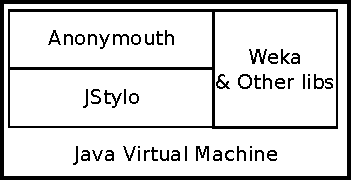
\includegraphics[width=0.4\textwidth]{img/jsan.pdf}
  \caption{Existing JSAN Architecture}
  \label{fig:jsan}
\end{figure}

\subsection{Requirements for Web Service}

The architecture for a web service imposes different requirements on
an application.  First and foremost, since Anonymouth is a privacy
enhancing technology, the web service \emph{must} not degrade the
privacy protection of the application.  This is a challenge when
migrating from a desktop to web service since the desktop application
does not use any networked communicaiton.  However, there is little
benefit to using Anonymouth on the web if it compromises one's
privacy.

\subsubsection{Low-latency.}
The web service as implemented is near-real-time, i.e. low-latency,
bounded primarily be the performance of Anonymouth. One key feature of
the current implementation is the asynchronous processing of
stylometric information, which allows a user to continually modify a
text while anonymity information is calculated in the background. The
latency of the response times for each stylometric analysis is on the
order of 1 to 2 minutes in the default configuration (see Performance
section for futher details).

A high latency system would not be well suited for a web service.  An
example high latency system could simply entail sending an encrypted
email to a third party who uses Anonymouth locally and returns the
encrypted result.  While this high-latency system seems trivial, note
that a naive implementation will reduce the user's privacy.  For
example, email is very subject to traffic analysis
\cite{Mathewson04practicaltraffic} and encrypted email is easy to
detect, therefore this act alone would raise suspiction.  If
this third party was offering a high-latency anonymiziation service
for numerous people, the network graph would be easy to detect.

\subsection{Architecture Qualities}
There are several qualities of a system architecture that are
considers foundational\cite{Bass:2012:SAP:2392670}.  These are: availability,
interoperability, modifiability, performance, security, testability,
and usability.  In additional we add privacy as an architecture
quality in our review.

Availability is the measure of the measure of the accesibility and
realibility of the system, e.g. how well does it handle errors.
Interoperability refers to the degree with which a system can interact
with its components or other systems.  Modifiability is important for
large systems so that they can be easily maintained and scale.  The
response of the system to input is its performance.  Security is the
review of a system's ability to protect sensitive data and prevent
unautorized and undesired behaviour.  Testability is an important
factor not only in development but also in a deployed system to ensure
that the system is working as designed.  Usability is notoriously bad
for security software \cite{Whitten:1999:WJC:1251421.1251435} and
refers to the interaction design.  Lastly, by privacy we mean how well
a user's anonymitity is protected.

In the following sections, we provide an analysis of each quality and
define the requirements for a stylometric web service.


\subsubsection{Availability.}

If the user can not access the web service, then the user is in the
same situation as having a device that can not run Anonymouth
locally.  The entry point to the web service requires a web server.
Realistically, this service will never see the traffic that FaceBook
or Twitter experiences, but the web server should be handle thousands
of requests per day.

A common attack to block availability is a Denial-of-Service (DoS)
attack.  A DoS attack is akin to receiving a momentarily burst in
traffic, i.e. the ``Slashdot effect.''  The difference lies in the
motivation for the sudden attention.  Thus, a service that is
resistant to DoS attacks also scales well to large second-derivative
increases in traffic.

There are many implemenation details to achieve availability that are
beyond the scope of this paper.  We attest that a stylometric service
needs to be available and should consider the effects of sudden
traffic increases.

\subsubsection{Interoperability.}

The stylometric web service we implemented is interoperable with the modern
web architecture.  Specifically, it should be a service based on
Representational State Transfer (REST)\cite{Fielding2000}.  REST web
services define a framework that is client-server, has a uniform
interface based on HTTP verbs, and supports a layered architecture.
These features are in-line with the goals of a stylometric web
service.  Using a REST service, the client software can be a web
browser, which is nearly ubiqiteious on mobile devices.

\subsubsection{Modifiability.}

One of the goals of the service is provide a platform for stylometric
research.  In this sense in must be modifable to accomodate different
kinds of experiments including ones not currently anticipated.
Software engineering best pratices are applicable here mainly having
well abstracted interfaces and modular components.  As a RESTful web
service, each endpoint should have a concise application programming
interface (API) for a given feature set.  For example, there should be
a stylometry endpoint that can process text and return features.
Other services, such as an adversarial stylometry service, should use
the stylometric service via its REST API.

A web service has a distinct advantage here over the modifiability of
the desktop software.  One can deploy an updated version of the
software by pushing the update to servers and instantly clients will
have the new version.  As a research platform, this is a very valuable
feature.  For example, split testing or A/B testing, is much easier to
control and manage with a web service than packaged software.

\subsubsection{Performance.}

We do not place an specific performance metrics on the service other
than that it should be reasonably responsive.  Since JStylo relies on
Weka \cite{Hall:2009:WDM:1656274.1656278} to implement the machine
learning algorithms, this server should have a decent amount of RAM.

\subsubsection{Security.}

The security features need for a stylometric service are
authentication, confidentiality, integrity, and repudiation.

{\bf Authentication.}  Users must be able to authenticate the
service.  We propose that if the service is using HTTPS with a server
certificate signed by a trusted certificate authority that this will
suffice.  However, when running behind a Tor Hidden Service, this is
slightly more complicated.  The service can sign the onion address
that it provides and Tor will ensure that the address maps to the
service.  The signature would correspond to a trusted certificate
authority issued certificate.  Mutual authentication, or
authentication of the users should \emph{not} be conducted as this
would either compromise the user's identity.

{\bf Confidentiality.} The service must protect the confidentiality of
the user's data.  The user is trusting the service with their corpus
and document to anonymize and that must be revealed to unauthroized
users.  However, one of the goals of this service is to allow multiple
authors to collaborate.  In this case, the confidentiality
requirements are more interesting.  We don't specifiy an
implementation, but there are various techniques that could satisfy
this requirement.

Besides multi-authors, the service is also multi-user.  Thus, the
user's document is loaded into RAM with other user's documents.
Therefore, the service is vulnerable to memory dump attacks.  Assuming
that the service runs on a third party provide, like Amazon Web
Services, it is also vulnerable to malicious insiders
\cite{conf/dsn/RochaC11}.

{\bf Integrity.}  The service must maintain the integrity of the
corpus and the target document.  This not only includes integrity in
transit but also the integrity of the presented document to the user.
Using Transport Layer Security (TLS), the integrity is guaranteed
during transit.

{\bf Repudiation.}  The service must not assign long-term identity
to any operations.  Therefore, TLS connections must use ephemeral
keys to provide Perfect Forward Secrecy (PFS).  The service must not
maintain logs that will identify the target document, the corpus, or
the users of the service.

\subsubsection{Testability.}

The service must be modular in design to support testing of each
endpoint.  While adopting the full Netflix-like approach may be
over-engineering for this limited web-service,
\cite{Tseitlin:2013:AO:2492007.2492022}, there are certainly aspects
of their design that are applicable.  For example the service should
be resilient to service outages.  If the service is unavailable, it
can not protect the anonymity of authors.

\subsubsection{Usability.}

\subsubsection{Privacy.}

\subsection{Example Architecture}

\begin{figure*}
  \centering
    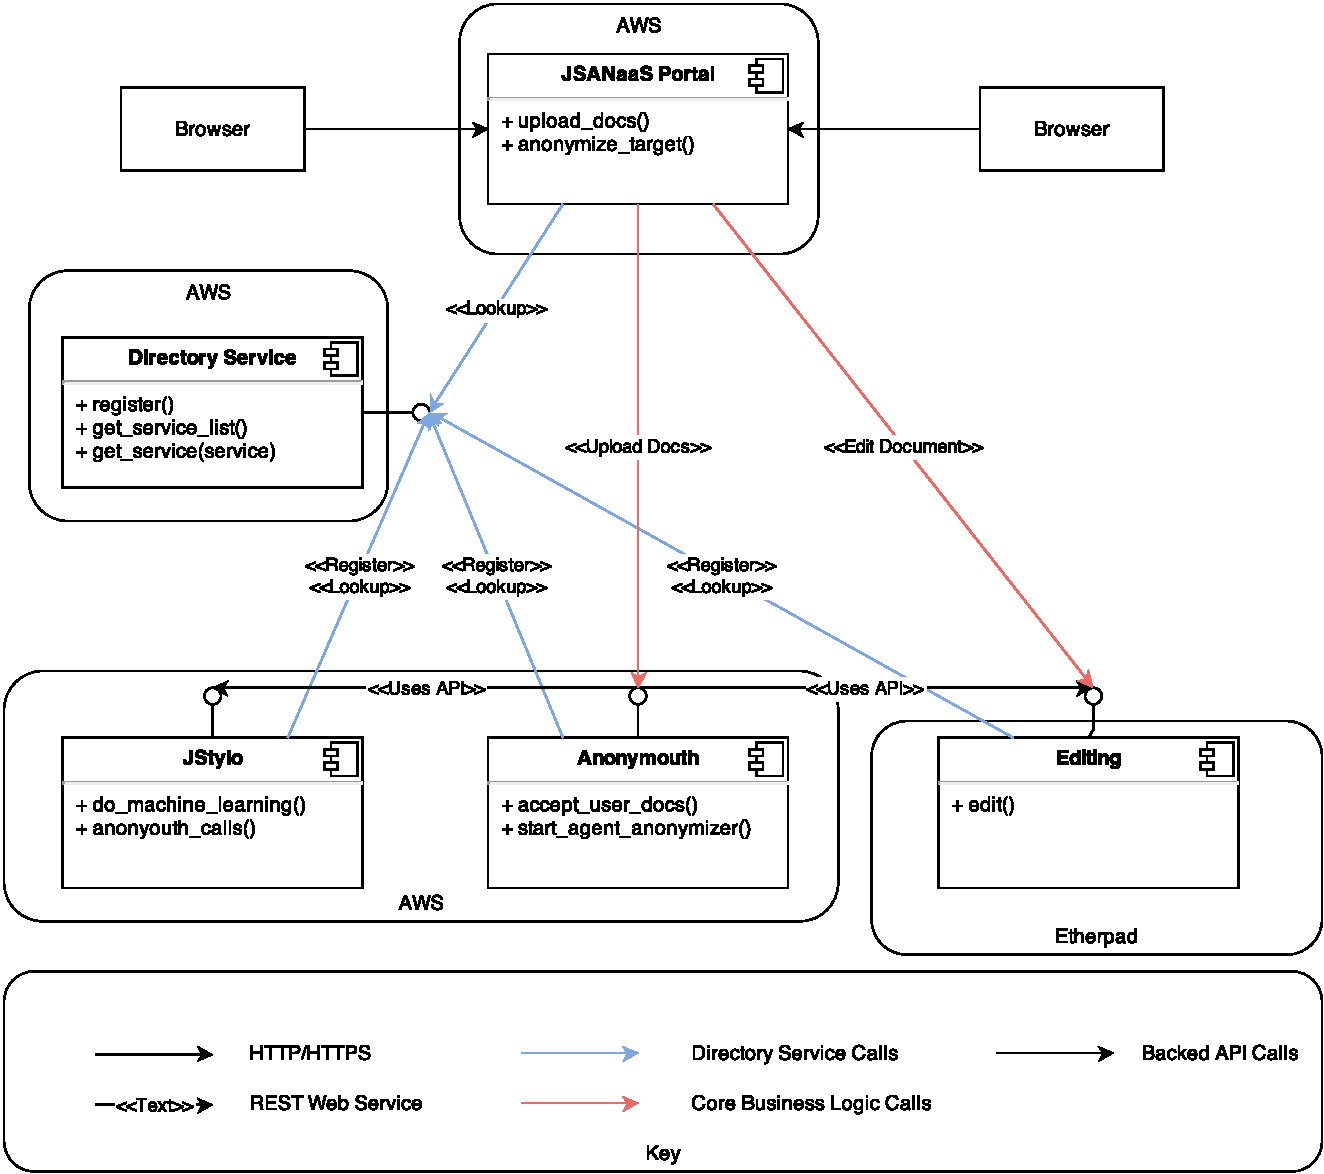
\includegraphics[width=0.6\textwidth]{img/jsanaas.pdf}
  \caption{Example JSANaaS Architecture as a Deployment Diagram}
  \label{fig:jsanaas}
\end{figure*}
\section{Security Analysis}

A number of attack vectors for the web application currently exist. We
discuss those which seem most significant here below. However one key
security implication of a web-delivered Stylometry Service is that it
is expected to be delivered over the web, can be accessed in this
configuration by anyone with knowledge of its unique URL (or .onion
address). This allows adversaries greater opportunity to attempt to
penetrate the security of the web application relative to a client
application installed on a PC that is not internet connected.

It is expected that, before the service would be used in a real-world
use case, a user would configure and deploy supporting databases
associated with the login and SSL options available in the
Play Framework.

Although web accessbility may be a significant risk from a usability
standpoint, the anecdotal infrequency with which adversarial
stylometry software is used even among privacy-conscious users as
determined by conversations with colleagues of the authors
suggests that delivery of this functionality via a web page (or even
potentially via a browser plugin functional across multiple web pages)
may be an appropriate trade-off to make.

Beyond the concerns mentioned above, a number of specific attack
vectors remain for a stylometric web service in general and for our
implementation in particular:

{\bf Man in the middle attacks}: If a user accepts a rogue SSL
certificate, it may be possible to create a "man in the middle" attack
where the user believes she is communicating with a specific
Stylometry Service, but is infact communicating via an impersonated
target.

{\bf Replay attacks}: An evesdropper may replay a message to the
webservice in an attempt to surrepituously revert parts of the text to
earlier versions. This may be possible as it is not documented whether
the current implementation uses nonces when transmitting messages.

{\bf HTML5 Canvas attacks}: The etherpad implementation uses the new
'canvas' element introduced in HTML5 extensively. Recently an attack
has been documented \cite{BrowserTiming} whereby Firefox optimizations
in the implementation of the requestAnimationFrame method have been
used by to detect differences in link coloring across frames (allowing
an adversary to determine if a particular styometry service has been
visited, for instance).

Note: We do not know if any of these vectors allows for a specific
attack, but suggest they should be considered for any future
implementation research in the area of stylometric web services using
a similar architecture.

\section{Privacy and Anonymity Analysis}

The privacy of a user accessing the web service is expected to be
ensured via the use of TLS/SSL encryption for all data transmitted
between the client and server. The anonymity of the user is expected
to be promoted via the use of an Onion Routing protocol such as Tor,
to ensure that the IP of the client cannot be directly linked to the
IP of the service.

\section{Implementation Details}

We implemented a web application based on the Play Web Application
Framework in Java. This web application had a reference to a modified
version of JSAN which was forked from the PSAL Anonymouth repository
\cite{PSAL:github}. In addition the application has major dependencies
on JQuery, Twitter Bootstrap (for page layout), and Etherpad (an
open-source collaborative text editing web application and library)
\cite{etherpad}. Etherpad (specifically Etherpad Lite is the version
used here) in turn has major dependencies on node.js for building and
running the backend service.

At a high level the implementation is as follows: A user browses to
the Stylometry Service via a web browser. This causes the Play
Framework web application to serve up a web page with an Etherpad
control and instructions for the user to enter in the document they
wish to anonymize. The etherpad control is implemented as an iframe
which serves an Etherpad that is connected to the node.js server
running the Etherpad backend (both servers should reside on the same
domain, running on different ports). The page served by Play also
contains a button which allows the author to specify when he or she
would like to submit the document for anonymization to
Anonymouth. Because the Anonymouth analysis process depends on a
number of computationally-intensive algorithms (among them running SMO
analysis in Weka as well as a Basic-9 feature stylometric analysis) we
implemented this calculation asynchronously. When a user clicks the
button to run an analysis, JQuery is used to issue a HTTP POST
containing in the message body a JSON-encoded representation of the
current Etherpad text to an endpoint at
\url{/getAnonymouthInfoJSON}. During the time that the Anonymouth
analysis is underway, a spinner control from the spin.js library is
used to indicate to the user than an analysis is underway. The fact
that the request is made to Anonymouth asynchronously allows a user to
continue editing the text while an analysis is running, allowing for a
smooth user experience.

The web service as implemented currently supports only 1 author as the
assumption is made that the author has pre-configured the "doc set"
(also referred to as 'problem set' in Anonymouth source) that provides
references as to the author's own writing style, as well as writing
samples for other authors that will be used as a reference for writing
styles that are different than that of the active author. The user can
additionally configure the anonymouth properties file
(\texttt{anonymouthprop.prop}) in the jsan resources directory to influence
settings such as the feature set to use for stylometric identification
as well as the number of threads to use and maximum number of features
to analyze.

One configured, the call to the \texttt{getAnonymouthInfoJSON} input
will overwrite the "test.txt" file on disk that is configured in the
provided problem set. This will ensure that changing the document in
Etherpad forces an update to the test file and thus ensuring that the
'latest' document is always anonymized. Once the problem set has been
updated, the 'Anonymouth library' is invoked. The 'Anonymouth library'
is a forked version of the current Anonymouth application, which is
designed to be used behind a Swing/AWT rich client GUI. A number of
implementation challenges were present when trying to separate the
core anonymization logic of Anonymouth from its GUI implementation -
most specifically, although an 'engine' namespace exists which holds
much of the anonymization logic, significant dependencies still
existed between the 'engine' and the 'GUI' namespaces, specifically in
the event handlers associated with the Editor screen and the
\texttt{GUIMain} classes. Much of the work in this project consisted
of reducing the coupling between these two namespaces.

As much of the configuration logic was handled at the GUI layer (via
\texttt{ThePresident} and \texttt{GUIMain} classes) we took the
approach of refactoring the GUI layer to work in a 'headless' mode,
that is, without any windows launching. Long-term it would be
preferable to have no dependencies on the GUI namespace at all for the
Stylometry Service, however this could not be achieved in the
available timeframe for this project. The web service thus invokes a
modified version of the \texttt{ThePresident} class, which coordinates
reading configuration files, loading the configured problem set, and
using numerous libraries (JGAAP and Weka among them) to conduct an
adversarial stylometric analysis. The results are returned by the web
service in the form of a JSON-encoded list of words to remove, as well
as an indication of 'changes needed' to the current text to reach an
acceptable level of anonynmity.

While this analysis has been running, the UI has been waiting on a
response to the request made of the Stylometric Service. Once this
request is returned, a request is made to spin.js library to stop the
spinner, and JQuery is again used to update a div on the page with the
results of the adversarial stylometric analysis. The JQuery Promises
interface was used to ensure that the UI correctly waited for these
otherwise asynchronous requests to be completed in the right order.

The web application (bundled with all dependencies) can be downloaded
as shown in Listing \ref{lst:download}.

\begin{lstlisting}[caption={Download Web Application},label={lst:download}]
git clone https://github.com/LRParser/anonymouth.git
./bootstrap.sh
\end{lstlisting}

This command will copy the latest JSAN JAR files to the \texttt{lib}
directory of the Play Framework Web Application, start a Play
Framework Server on port $9000$, and start an Etherpad Lite server on
port $9001$ over node.js.

\section{Comparison to Stand-alone Application}

The stand-alone application has both advantages and disadvantages
relative to the web service. To start with advantages: it contains
more robust error handling, offers a GUI to create a problem set, and
provides a richer editing experience for anonymized
texts. Disadvantages concern ease of use (users must download and
execute a JAR file) and supported platforms (it is unlikely that this
JAR file will be supported on many mobile phones, for instance). The
Stylometry Service, in contrast, is potentially more accessible than
the standalone application: it can be accessed via mobile phones and
tablets, for instance. Likewise application delivery may be simpler -
nothing must be downloaded locally. Furthermore, the web application
maintains a 'timeline' of changes made to a text and also allows for
simple multi-party anonymization of documents.

Disadvantages to the web application include the fact that it offers
fewer anonymization features (for instance, highlighting of specific
text passages), instead focusing primarily on 'words to
remove'. Furthermore, its security footprint is less well known, as it
introduces a number of new dependencies / potential attack vectors
such as JQuery, Twitter Bootstrap, Etherpad Lite, node.js, etc.

For a user likely to be using mobile devices or a casual user looking
to quickly anonymize texts, we suggest that the web interface may be a
better option. For a user facing a highly sophisticated adversary and
needing detailed anonymization suggestions, we suggest that the
stand-alone application may be a better option. We note that there is
no technical reason that could keep the web application from offering
all of the same anonymization suggestions as the standalone
application, and thus is may be the case that in the future the web
application could be recommendable to a wider range of users.
standalone client

\section{Deployment}

The web application can be deployed on a Ubuntu 12.04 desktop
installation per Listings \ref{lst:install} and \ref{lst:start}.

\begin{lstlisting}[caption={Install Dependencies},label={lst:install}]
sudo apt-get update
sudo apt-get install ubuntu-desktop ant openjdk-7-jdk postgresql git
sudo add-apt-repository ppa:chris-lea/node.js
sudo apt-get update
sudo apt-get install nodejs
git clone https://github.com/LRParser/anonymouth.git
\end{lstlisting}

\begin{lstlisting}[caption={Start Service},label={lst:start}]
cd anonymouth
./bootstrap.sh
\end{lstlisting}

\section{Single User Evaluation}

Although time didn't permit detailed user testing of the web
application, the authors did conduct one experiment with two users
using Amazon Mechanical Turk. Users were given 45 minutes to anonymize
a document. The title of the request was "Help re-phrase approx. 500
word texts as part of a research project". Specifically users were
asked, 'Re-phrase the text in the below-linked document while keeping
the original meeting. Substitute synonyms, change punctuation (I am to
I'm), split up / join sentences, etc. This is part of a research
project to see how well different persons can make a text appear as if
it wasn't written by the original author.'

The responses of users on Mechanical Turk (who were trying to
anonymize a text without any supporting software) were compared with
anonymization attempts by the authors of this paper against the same
document. The anonymization attempts by the authors took place before
reviewing the submissions from Mechanical Turk. For one sample paper,
d \texttt{09.txt} from the Brennan-Greenstadt corpus \cite{BrennanG09}
, we noted that Anonymouth returned a "changes needed"
score on the original document of $2.518$, $2.677$ for the users 'naive'
attempt to anonymize over Mechanical Turk, and $2.467$ for the attempt
of one of the authors to anonymize using the web application created
in this paper. Each of the two anonymization attempts for the 500-word
document took approximately 15 minutes. Although these results are far
from achieving statistical significance, they do suggest that it may
be possible to use this software to achieve anonymization levels which
surpass those of a 'naive' anonymization attempt.

\section{Multiple Concurrent User Evaluation}

TODO

\section{Evaluation of Architecture Qualities}

\subsection{Performance.}

The performance of the Stylometry Service as implemented is largely
determined by that of the Anonymouth service that it uses to get
stylometry suggestions. For an analysis of 1 500-word test document vs
23 documents from 4 'other' authors and using 8 training documents
from the to-anonymize author, we recorded a total of 67 seconds
required for the Anonymouth analysis, with less than 1 additional
second used to update the client UI, on a 3.3 Ghz Core i5 Ubuntu 12.04
Desktop machine, using 1 calculation thread for Anonymouth. These
results suggests that any attempts at performance optimization should
center around optimizing the performance of the Anonymouth
configuration.

After each stylometric analysis is complete, the web service ensures
all relevant anonymouth resources are closed. This allows the web
service to be used over a long period of time (20 or more
anonymization attempts have been tested) without memory leaks noted.

Further performance testing and optimization is required in order to
support a true multi-user service. The authors would suggest using a
web service based load test framework, such as Apache's JMeter or
LoadUI, in order to fully test the service under various potential
user loads.

\subsection{Testability.}

The web service UI is amenable to automated testing via web testing
frameworks such as Selenium (although such tests were not written for
this project). JUnit tests, in contrast, were written to test both
service method paths implemented. The authors consider the fact that
this application is delivered as a web application with a distinct
service layer to be a positive from the standpoint of testability, as
it allows users who may wish to modify the service the ability to
expand an existing unit test suite.

\section{Conclusion}

There are two significant contributions as a result of this work.  The
first is a stylometric web service.  This advances the usability
and capabilities of JSAN and provide a framework for more expansive
user testing in the future. The user testing results suggest that a
web interface may offer usability advantages while still providing a
meaningful increase in author anonymity.  The second contribution is that this is
the first framework for multi-author adversarial stylometry.  Our
results here suggest TODO.

\section*{Related Work}\label{sec:related}
This proposal extends the work from Drexel's PSAL, who have made
several contributions in this field.  In
\cite{conf/pet/McDonaldACSG12}, the authors present the Anonymouth
framework for anonymizing writing.
\cite{Afroz:2012:DHF:2310656.2310711} confirmed adversarial stylometry
is very effective at obfuscated authorship, but also presented
techniques to hide the prescience adversarial stylometry.  Lastly,
\cite{journals/tissec/BrennanAG12} presented successful adversarial
stylometry techniques through obfuscation, imitation, and translation
and produced two corpora of texts.

Tor is one of the most successful anonymity services in
operation \cite{Dingledine04tor:the}.  We intend to protect the
anonymity of users by offering JSAN over a Tor hidden service
however, there has been recent research de-anonymizing popular hidden
services \cite{oakland2013-trawling}.  We will provide a discussion on
the design and experience of enabling a hidden service, but we will
focus on this aspect.

\begin{table}
  \centering
  \begin{tabular}{l | c}
    Milestone & Date\\
    \hline

    Document initial design & October 28\\
    Finish porting JSAN to a web service & November 4\\
    Add the Firebase editro & November 11\\
    Add the third party feature & November 18\\
    Conduct evaluation & November 25\\
    Provide Paper and Presentation & December 2

  \end{tabular}
  \caption{Project Milestones}
  \label{tab:milestones}
\end{table}


\subsection*{Future Work}

The scope of this project is designed to completed in one Drexel
quarter, however we have several ideas for continued work.  With a web
service, we can offer real-time adversarial stylometry.  Assume Alice,
who has a blog, wants to anonymize her next blog post.  She would
connect to our web service, submit the URL for her blog and then write
her next post with adversarial stylometry.  This real-time data
crawling at this scale is simply not feasible with stand alone
software.

Now that a third party will be re-writing documents, we feel that it
is important to obfuscate the content from the re-writer.  One idea,
is to mix the document, perhaps with other documents, prior to
re-writing.  The re-writer would be presented with an otherwise
nonsensical document and would focus on re-write each sentence in her
native style.  The combined document, would contain $n$ author styles,
where $n$ is the number of re-writing authors.

Lastly, for long term adversarial projects, we are curious on how often
one has to re-train the model.  We imagine that a web service could
help monitor the change of a stylometric fingerprint over time.


%%%%%%%%%%
% References and End of Paper
\bibliography{service}
\bibliographystyle{aaai}


\end{document}
%%% Local Variables
%%% mode: latex
%%% TeX-master: t
%%% End:
